\documentclass[a4j, titlepage]{jarticle}

\usepackage[dvipdfmx]{graphicx}

\usepackage{subcaption}

\makeatletter
\newcommand{\figcaption}[1]{\def\@captype{figure}\caption{#1}}
\newcommand{\tblcaption}[1]{\def\@captype{table}\caption{#1}}
\makeatother

\title{\LaTeX で図表を使う}
\date{\today}
\author{自分の名前}

\begin{document}
  \maketitle

  \tableofcontents
  \clearpage


  \section{はじめに}
  今回は \LaTeX で図や表を扱う方法を学ぶ.
  レポートや論文などでも, 実験結果の図(グラフ)や表を載せなければ説得力がない.
  これまでと比べて少し癖のある構文にはなるが, しっかりとコマンドを身につけよう.


  \section{表の書き方}
  
  \begin{table}[htb]
    \caption{C言語の代表的なデータの型}
    \label{table:data_type}
    \begin{center}
      \begin{tabular}{lcr}
        \hline
        データの型  & 宣言  &  ビット幅[bit]  \\
        \hline
        \hline
        文字型  & char  & 8 \\
        整数型  & int   & 32 \\
        倍精度実数型  & double  & 64 \\
        倍々精度実数型  &  long double  &  96 \\
        \hline
      \end{tabular}
    \end{center}
  \end{table}

  表\ref{table:data_type} は, C言語で用いられるデータの型とビット幅の関係を表したものである.

  表\ref{table:bubble}に, バブルソートの各データに対するデータ数100,000個の時の実行時間(10回平均)を示す.

  \begin{table}[htb]
    \caption{バブルソートの各データに対するデータ数100,000個の時の実行時間(10回平均)}
    \label{table:bubble}
    \begin{center}
      \begin{tabular}{|l|c|}
        \hline
        \multicolumn{2}{|c|}{バブルソートの実行時間(10回平均)}\\
        \hline
        \hline
        \multicolumn{1}{|c|}{データファイル名} & 実行時間[s]\\
        \hline
        data1.dat (ランダムデータ) & 26.2918089000\\
        \hline
        data2.dat (ランダムデータ) & 26.3672766000\\
        \hline
        data3.dat (ランダムデータ) & 26.3093366000\\
        \hline
        data4.dat (昇順データ) & 10.0458130000\\
        \hline
        data5.dat (降順データ) & 18.4367828000\\
        \hline
        data6.dat (バイトニックデータ) & 14.2316616000\\
        \hline
        data7.dat (ジグザグデータ) & 23.2754890000\\   
        \hline
      \end{tabular}
    \end{center}
  \end{table}

  \clearpage
  

  \section{図の表示方法}

  \begin{figure}[htb]
    \begin{center}
      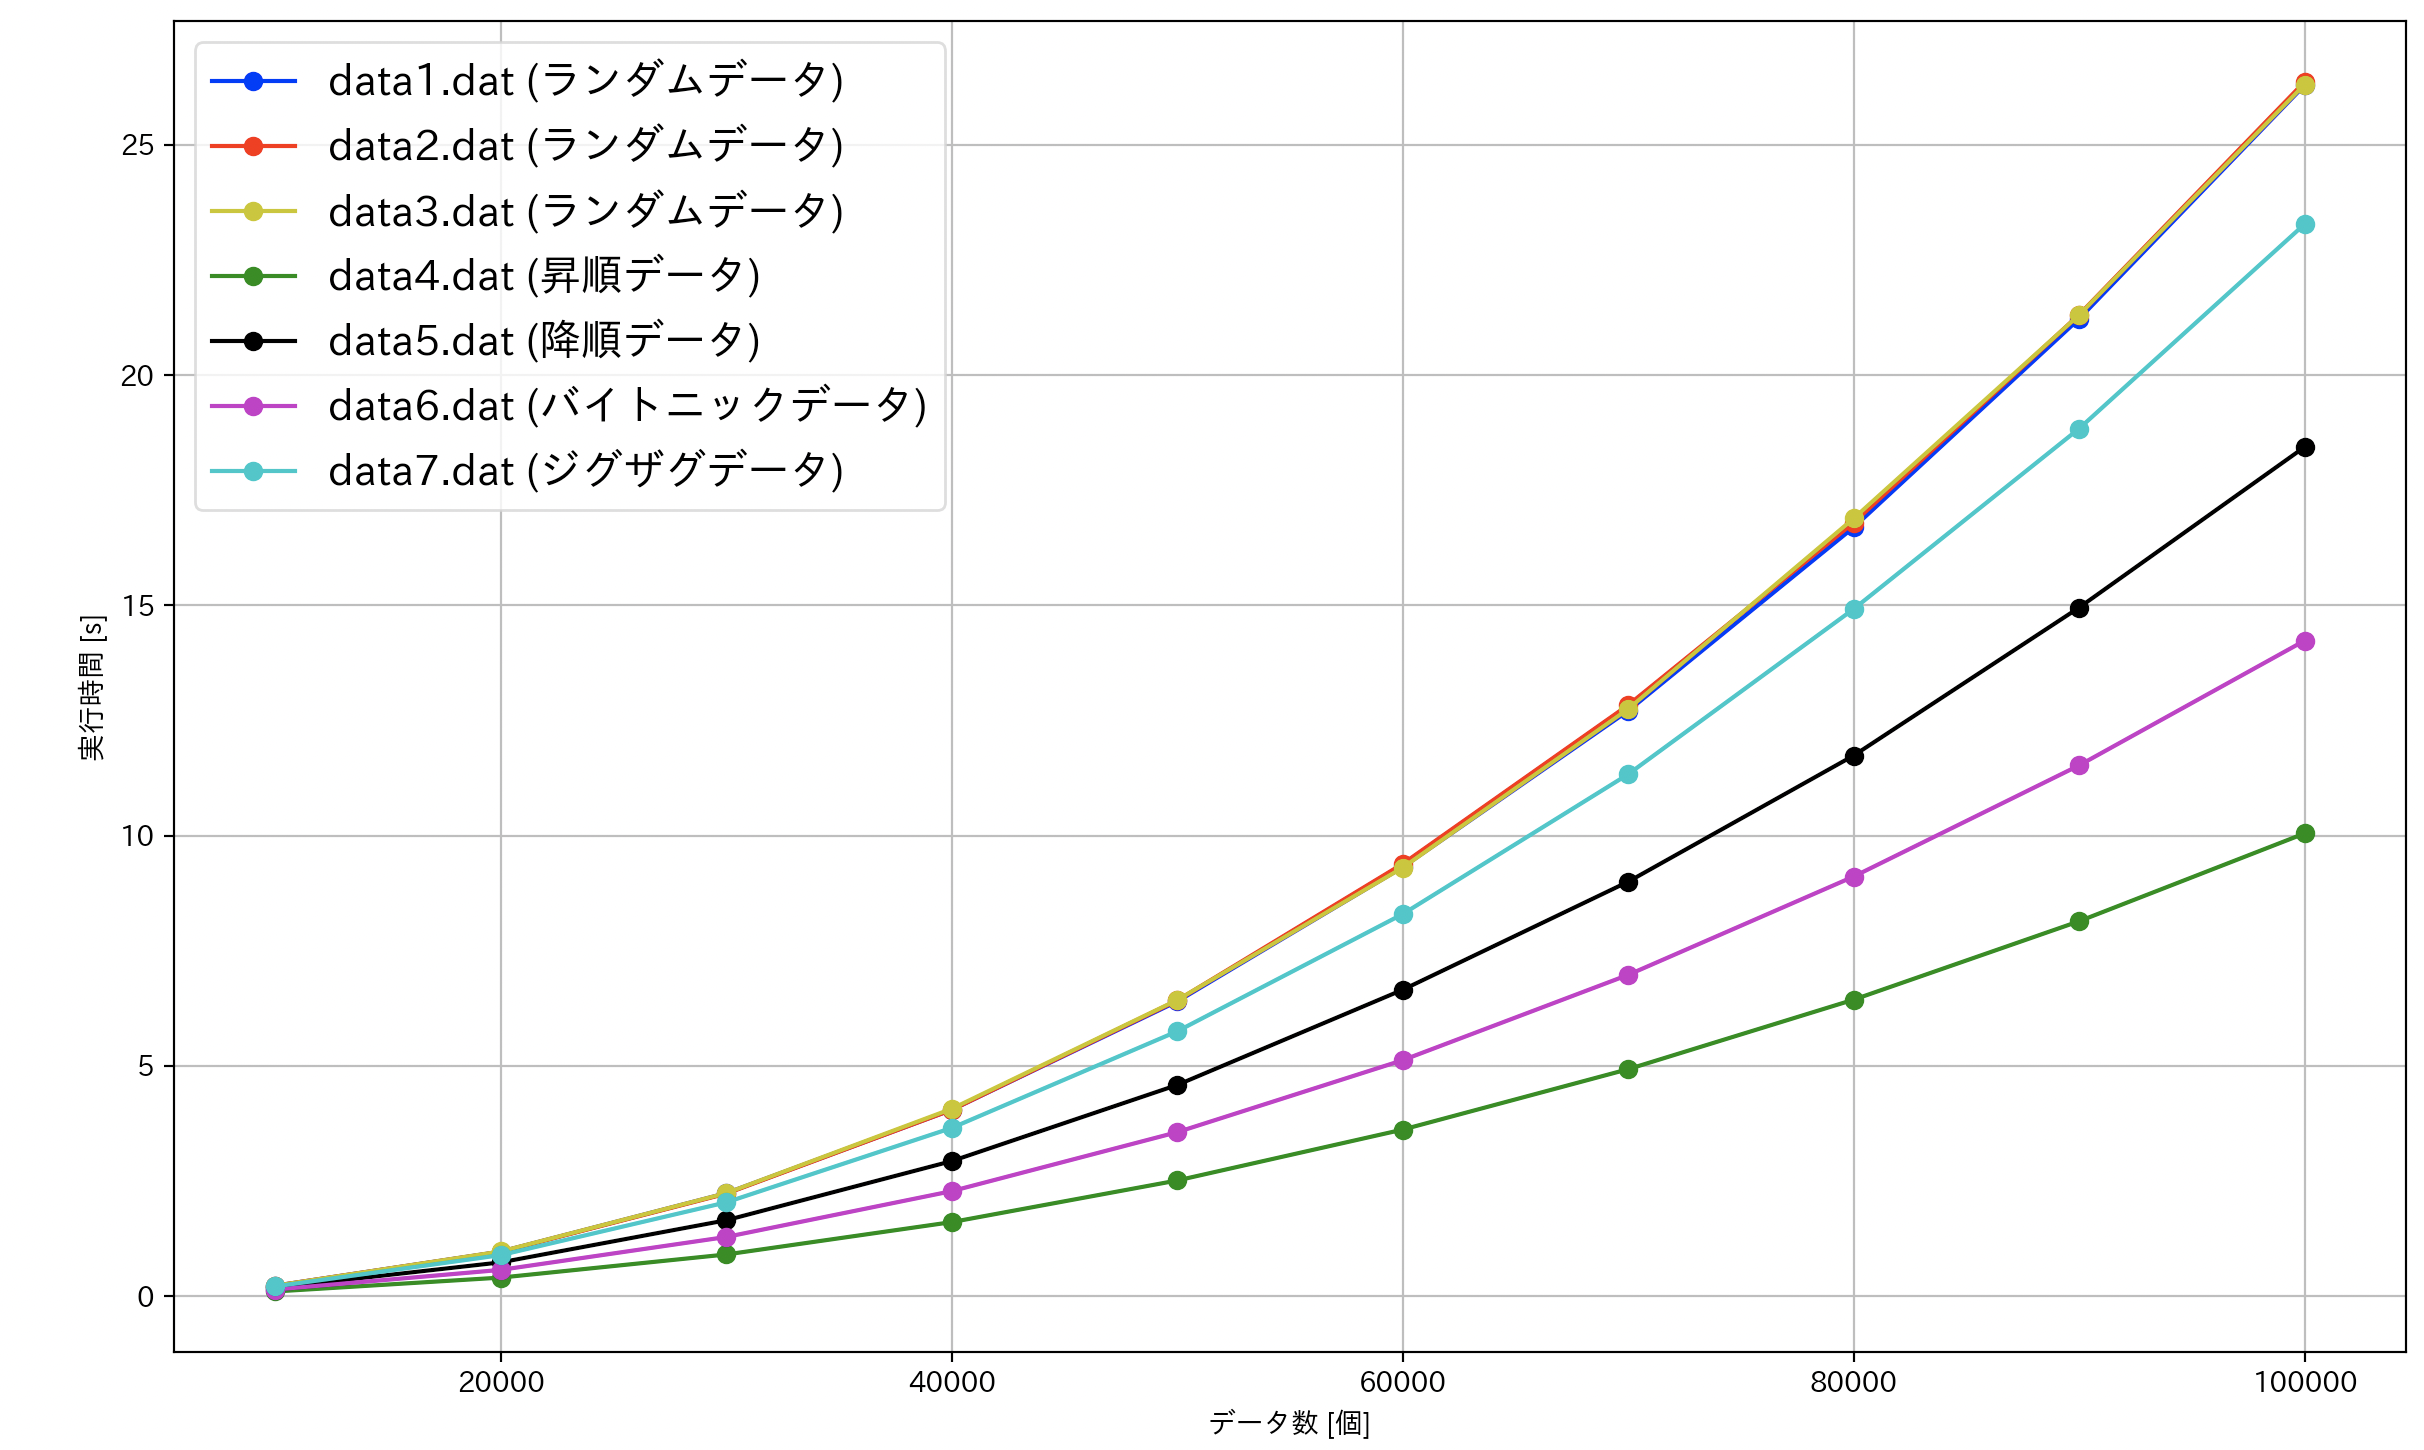
\includegraphics[scale=0.3]{bubble.png}
      \caption{バブルソートの各データに対するデータ数と実行時間 (10 回平均) の関係}
      \label{graph:bubble}
    \end{center}
  \end{figure}

  \ref{graph:bubble} より, バブルソートのアルゴリズムの計算量は$O(n^2)$であることが考えられる.


  \section{画像と表を横に2つ並べる}

  \begin{figure}[htb]
    \begin{minipage}{0.4\textwidth}
      \begin{center}
        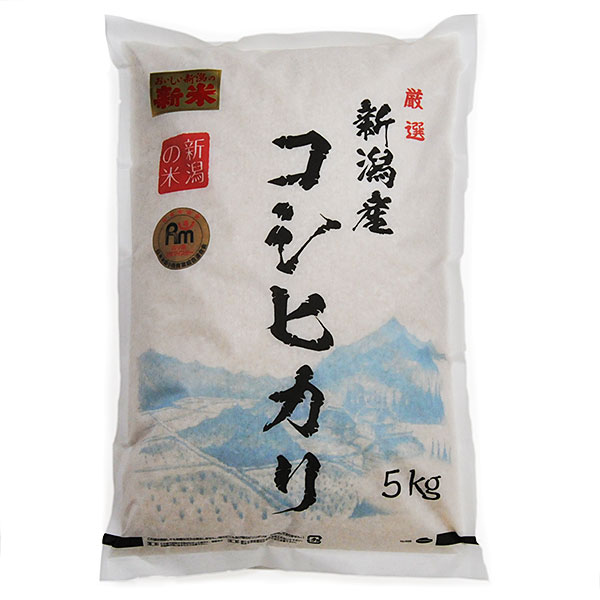
\includegraphics[scale=0.2]{koshihikari.jpg}
        \caption{新潟県のブランド米}
        \label{image:koshihikari}
      \end{center}
    \end{minipage}
    \begin{minipage}{0.5\textwidth}
      \begin{center}
        \makeatletter
        \def\@captype{table}
        \makeatother
        \tblcaption{米の収穫量ランキング 令和3年産水稲}
        \label{table:rice}
        \begin{tabular}{|r|l|r|}
          \hline
          順位 & 道県名 & 収穫量[t]\\
          \hline
          \hline
          1 & 新潟県 & 620,000\\ 
          \hline
          2 & 北海道 & 573,700\\ 
          \hline
          3 & 秋田県 & 501,200\\ 
          \hline
          4 & 山形県 & 393,800\\
          \hline
          5 & 宮城県 & 353,400\\
          \hline
        \end{tabular}
      \end{center}
    \end{minipage}
  \end{figure}

  表\ref{table:rice} は令和3年度の米の収穫量ランキング~\cite{Rice01}であり, 図\ref{image:koshihikari} は新潟県のブランド米のひとつである.
  米の1人当たりの年間消費量は, 昭和37年度をピークに118kgであったが, 令和2年度では50.8kgと昭和37年度の半分以下にまで減少している.~\cite{Rice01}
  このような状況において, 国では米の消費拡大に向けて, 米飯学校給食の推進や健康面からのごはん食の効用の発信などを実施している.
  \begin{thebibliography}{99}
    \bibitem{Rice01}
    "農林水産省". https://www.maff.go.jp/, (参照 2022-12-16).
  \end{thebibliography}

\end{document}